% SC2008 --- Chapter 5: Network Layer -- IP, Forwarding, Dijkstra, BGP (0->100)
\chapter{Network Layer: IP, Forwarding and Routing}\label{ch:network-ip}
\begin{quote}
\emph{``The network layer glues billions of links into one Internet.''} --- IP promises only best-effort delivery; routing makes the promise useful by finding paths at planetary scale.
\end{quote}
\noindent\fbox{\parbox{\dimexpr\linewidth-2\fboxsep-2\fboxrule}{%
\textbf{From zero: we build here, no prior networking assumed.} We start from ``how does a packet cross many networks?'' with pictures before headers or algorithms. Every notion---datagram, prefix, forwarding table, shortest path, autonomous system---is defined on first use. No IP or graph-theory background is needed beyond basic sets.}}
\vspace{0.4em}
\section*{Learning Outcomes}
After this chapter you will be able to:
\begin{enumerate}[label=(L\arabic*)]
    \item describe the IPv4 datagram format, addressing, CIDR and subnetting;
    \item distinguish forwarding (data plane) from routing (control plane) and apply longest-prefix match;
    \item execute Dijkstra's link-state algorithm and prove its correctness invariant;
    \item compare link-state vs.\ distance-vector (Bellman--Ford) and count-to-infinity;
    \item explain BGP as path-vector inter-domain routing: ASes, peering, and policy.
\end{enumerate}
% ============================================================
\section{Why a Network Layer?}\label{sec:why-network}
Transport gives end-to-end reliability between hosts, but who moves a packet \emph{across} many networks? The network layer does. Think of a postal system: you write a destination address on the envelope (IP address); each post office (router) looks only at the address and forwards it toward the destination. The sender need not know the full route.
Two planes: \emph{data plane} (per-packet forwarding in hardware, nanoseconds) and \emph{control plane} (computing forwarding tables, milliseconds to minutes). IP is the narrow waist---everything over IP, IP over everything. Without a network layer, every pair of networks would need a custom gateway; with IP, $N$ networks need only $N$ IP interfaces, not $N^{2}$ translators.
\section{IPv4 Datagram and Addresses}\label{sec:ipv4}
An IPv4 datagram carries a 20-byte header (plus options) and payload.
\begin{center}
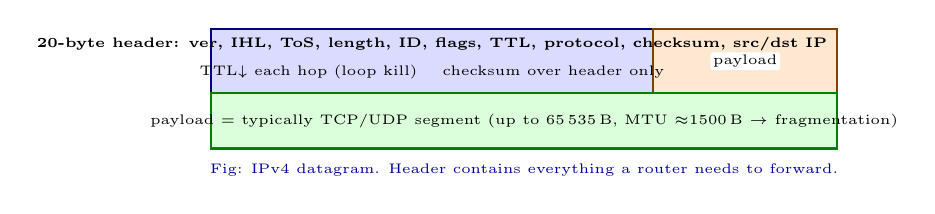
\begin{tikzpicture}[scale=0.78, every node/.style={font=\scriptsize}]
\draw[fill=blue!14, draw=blue!50!black, thick] (0,0) rectangle (7.2,1.05);
\draw[fill=orange!18, draw=orange!50!black, thick] (7.2,0) rectangle (10.2,1.05);
\draw[fill=green!14, draw=green!50!black, thick] (0,-0.9) rectangle (10.2,0);
\node[font=\tiny\bfseries] at (3.6,0.80) {20-byte header: ver, IHL, ToS, length, ID, flags, TTL, protocol, checksum, src/dst IP};
\node[font=\tiny] at (3.6,0.35) {TTL$\downarrow$ each hop (loop kill) \quad checksum over header only};
\node[font=\tiny, fill=white, rounded corners=1pt, inner sep=1pt] at (8.7,0.52) {payload};
\node[font=\tiny] at (5.1,-0.45) {payload = typically TCP/UDP segment (up to 65\,535\,B, MTU $\approx$1500\,B $\to$ fragmentation)};
\node[font=\tiny, blue!60!black] at (5.1,-1.25) {Fig: IPv4 datagram. Header contains everything a router needs to forward.};
\end{tikzpicture}
\end{center}
Addresses are 32-bit, written as dotted decimal: $192.168.1.10 = 11000000.10101000.00000001.00001010$. Originally classful (A/B/C); now \emph{CIDR}: $a.b.c.d/x$ means first $x$ bits are network prefix, rest host. Example: $203.0.113.0/24$ leaves $2^{8}=256$ addresses. A host with $/26$ has subnet mask $255.255.255.192$. Longest-prefix matching (next section) makes CIDR aggregation possible---ISP advertises one $/16$ instead of 256 $/24$s. IPv6 fixes exhaustion with 128-bit addresses (hex, e.g.\ \texttt{2001:db8::1}), same forwarding idea.
\begin{definition}[Subnet]\label{def:subnet}
A \emph{subnet} is a set of interfaces with a common prefix whose packets can be delivered without a router (shared link or switched LAN). A host's address has network part (prefix) and host part.
\end{definition}
CIDR aggregation: an ISP holding $14.24.0.0/15$ covers $2^{17}=131\,072$ addresses---range $14.24.0.0$ to $14.25.255.255$, i.e.\ two adjacent $/16$s. Without aggregation the global BGP table would exceed $800$k entries; with CIDR it stays manageable. On a host, $/26$ means $64$ addresses ($62$ usable) with mask $255.255.255.192$.
Fragmentation: if payload $>$ MTU, router/host splits into fragments sharing the same ID. Example: 4000\,B datagram over MTU 1500 $\to$ fragments 1480+1480+1040 payload (20\,B header each, offset in 8\,B units, MF flag). Reassembly only at destination---avoided today via Path MTU Discovery (sender probes with DF bit, learns bottleneck MTU). IPv6 forbids router fragmentation entirely.
Header fields matter: TTL (now hop limit) prevents loops---each router decrements, drops at zero and sends ICMP Time Exceeded (basis of \texttt{traceroute}). Protocol field demultiplexes to TCP (6), UDP (17), etc. Header checksum is recomputed each hop because TTL changes; IPv6 drops it (link layers already check).
\section{Forwarding: Longest-Prefix Match}\label{sec:forwarding}
Each router stores a \emph{forwarding table}: $(\text{prefix}, \text{link})$ pairs computed by routing protocols. On arrival, it finds the \emph{longest} prefix matching the destination IP and forwards on that link. Default route $0.0.0.0/0$ catches the rest. Forwarding is per-datagram, stateless, and must be fast---core routers handle $>100$M lookups/s via TCAM or trie in ASIC.
\begin{figure}[h]
\centering
\resizebox{\linewidth}{!}{%
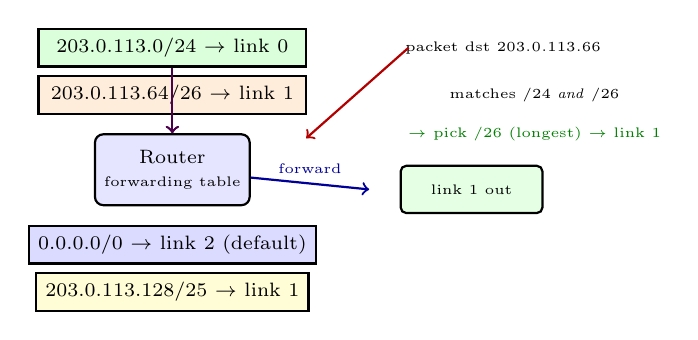
\begin{tikzpicture}[every node/.style={font=\scriptsize},
  tbl/.style={draw, thick, minimum width=3.4cm, minimum height=0.48cm, align=center},
  rtr/.style={draw, thick, rounded corners=3pt, fill=violet!10, minimum width=1.6cm, minimum height=0.9cm, align=center}]
\node[rtr, fill=blue!10] (R) at (0,0) {Router\\{\tiny forwarding table}};
\node[tbl, fill=green!14] (r1) at (0,1.55) {203.0.113.0/24 $\to$ link 0};
\node[tbl, fill=orange!14] (r2) at (0,0.95) {203.0.113.64/26 $\to$ link 1};
\node[tbl, fill=blue!14] (r3) at (0,-0.95) {0.0.0.0/0 $\to$ link 2 (default)};
\node[tbl, fill=yellow!16] (r4) at (0,-1.55) {203.0.113.128/25 $\to$ link 1};
\draw[->, thick, violet!60!black] (r1) -- (R);
\draw[->, thick, violet!60!black] (r2) -- (R);
\node[font=\tiny, fill=white, inner sep=1pt] at (4.2,1.55) {packet dst $203.0.113.66$};
\draw[->, thick, red!70!black] (3.0,1.55) -- (1.7,0.4);
\node[font=\tiny, align=left] at (4.6,0.95) {matches /24 \emph{and} /26};
\node[font=\tiny, align=left, green!50!black] at (4.6,0.45) {$\to$ pick /26 (longest) $\to$ link 1};
\draw[->, thick, blue!60!black] (R) -- (2.5,-0.25) node[midway, above, font=\tiny] {forward};
\node[draw, thick, fill=green!10, rounded corners=2pt, minimum width=1.8cm, minimum height=0.6cm, font=\tiny] at (3.8,-0.25) {link 1 out};
\end{tikzpicture}}%
\caption{Longest-prefix match: $203.0.113.66$ matches both $/24$ and $/26$; the more specific $/26$ wins. Table lookups are done in hardware (TCAM) for millions of prefixes.}
\label{fig:lpm}
\end{figure}
This is why aggregation works: a less-specific route covers many destinations, overridden where needed by more specific ones. A binary trie on prefix bits implements LPM in software: walk bits from MSB, remember last matching prefix. Hardware TCAM matches all entries in parallel.
\begin{lstlisting}[language=Python]
def longest_prefix_match(dst_ip, table):
    """table: list of (prefix_int, mask_len, link). dst_ip: 32-bit int."""
    best_link, best_len = None, -1
    for pref, mlen, link in table:
        mask = ((1 << 32) - 1) ^ ((1 << (32 - mlen)) - 1) if mlen>0 else 0
        if (dst_ip & mask) == (pref & mask) and mlen > best_len:
            best_len, best_link = mlen, link
    return best_link

# Example: 203.0.113.66 = 0xCB007142
table = [(0xCB007100,24,0),(0xCB007140,26,1),(0,0,2),(0xCB007180,25,1)]
print(longest_prefix_match(0xCB007142, table))  # -> 1 (the /26)
print(longest_prefix_match(0xCB007190, table))  # -> 1 (the /25)
\end{lstlisting}
Forwarding vs.\ routing: forwarding is the \emph{act} (table lookup per packet); routing is the \emph{computation} (building that table via Dijkstra/BGP). Separation lets forwarding stay simple and fast while routing can be complex and distributed.
\section{Dijkstra: Link-State Routing}\label{sec:dijkstra}
How does the control plane \emph{fill} those tables? Each router must know shortest paths. Model the network as a weighted graph $G=(V,E)$, $c(u,v)\ge0$. Link-state protocols (OSPF) flood each link's cost to all routers, so every router learns the full graph and runs Dijkstra locally.
\emph{Intuition first.} Stand at source $s$ and watch a wavefront expand at speed $1/c$. The first time the wave hits a node, it arrived via the shortest path---never improve later because all edges are non-negative. Dijkstra simulates this wavefront with a priority queue.
\begin{figure}[h]
\centering
\resizebox{0.95\linewidth}{!}{%
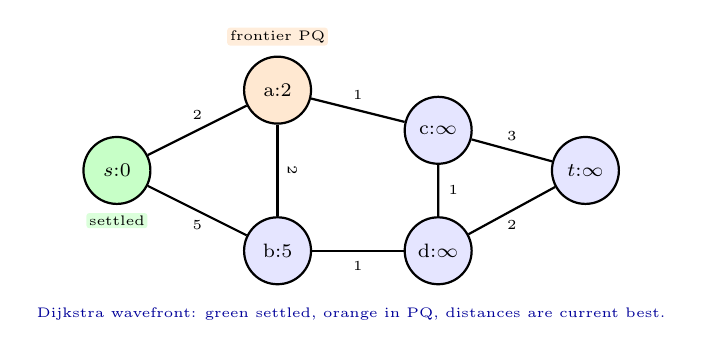
\begin{tikzpicture}[scale=0.85, every node/.style={font=\scriptsize},
  vnode/.style={circle, draw, thick, fill=blue!10, minimum size=0.85cm},
  done/.style={circle, draw, thick, fill=green!22, minimum size=0.85cm},
  frontier/.style={circle, draw, thick, fill=orange!18, minimum size=0.85cm}]
\node[done] (s) at (0,0) {$s$:0};
\node[frontier] (a) at (2.4,1.2) {a:2};
\node[vnode] (b) at (2.4,-1.2) {b:5};
\node[vnode] (c) at (4.8,0.6) {c:$\infty$};
\node[vnode] (d) at (4.8,-1.2) {d:$\infty$};
\node[vnode] (t) at (7.0,0) {$t$:$\infty$};
\draw[thick] (s)--node[above, font=\tiny] {2} (a);
\draw[thick] (s)--node[below, font=\tiny] {5} (b);
\draw[thick] (a)--node[above, font=\tiny] {1} (c);
\draw[thick] (a)--node[above, font=\tiny, sloped] {2} (b);
\draw[thick] (b)--node[below, font=\tiny] {1} (d);
\draw[thick] (c)--node[above, font=\tiny] {3} (t);
\draw[thick] (d)--node[below, font=\tiny] {2} (t);
\draw[thick] (c)--node[right, font=\tiny] {1} (d);
\node[font=\tiny, fill=green!14, rounded corners=1pt, inner sep=1pt] at (0,-0.75) {settled};
\node[font=\tiny, fill=orange!14, rounded corners=1pt, inner sep=1pt] at (2.4,2.0) {frontier PQ};
\node[font=\tiny, blue!60!black] at (3.5,-2.15) {Dijkstra wavefront: green settled, orange in PQ, distances are current best.};
\end{tikzpicture}}%
\caption{Dijkstra from $s$ after settling $s$: frontier $\{a(2),b(5)\}$. Next extract $a$, relax its edges. Edge weights $\ge0$ guarantee settling is final.}
\label{fig:dijkstra}
\end{figure}
\begin{lstlisting}[language=Python]
import heapq
def dijkstra(adj, s):
    """adj[u]=list of (v,w) w>=0. Returns dist, parent."""
    n = len(adj); INF = 10**18
    dist = [INF]*n; parent = [-1]*n
    dist[s]=0; pq=[(0,s)]
    visited=[False]*n
    while pq:
        d,u = heapq.heappop(pq)
        if visited[u]: continue
        visited[u]=True          # settled: d is final shortest distance
        for v,w in adj[u]:
            if dist[v] > d + w:  # relax
                dist[v]=d+w; parent[v]=u
                heapq.heappush(pq,(dist[v],v))
    return dist, parent

adj=[[(1,2),(2,5)],[(2,2),(3,1)],[(4,1)],[(4,3),(5,2)],[(5,1)],[]]
print(dijkstra(adj,0)[0])  # [0,2,4,3,5,6]
\end{lstlisting}
\emph{Invariant:} when $u$ is extracted, $\mathit{dist}[u]$ equals the true shortest-path distance $\delta(s,u)$. Proof by cut: any alternative path must cross from settled $S$ to $V\setminus S$ with cost $\ge \min$ frontier, so cannot beat $u$. The $w\ge0$ condition is essential---negative edges could offer a shortcut through unsettled nodes. Complexity $O((n+m)\log n)$ with binary heap; $O(m+n\log n)$ with Fibonacci heap. OSPF floods link states via LSAs so every router runs Dijkstra independently and consistently.
\section{Distance-Vector and BGP}\label{sec:dv-bgp}
\emph{Distance-vector} (Bellman--Ford) is dual: each node $x$ keeps $D_x(y)=\min_v\{c(x,v)+D_v(y)\}$ and exchanges vectors with neighbours. No global view; iterates to convergence in $O(nm)$ worst case. It underlies RIP (hop count, max 15).
\emph{Pitfall:} link cost increase can cause count-to-infinity. Example: $a$--$b$--$c$ line ($c=1$ each). If $b$--$c$ fails, $b$ thinks it can reach $c$ via $a$ (which routes through $b$!) and both increment slowly to infinity. Poisoned reverse (advertise $\infty$ back to next-hop) mitigates for two-node loops but fails on larger cycles---hence RIP limits diameter.
For Internet scale, no router can run Dijkstra on 100k networks. The Internet is federated into \emph{Autonomous Systems} (ASes---ISPs, campuses). \emph{BGP} (Border Gateway Protocol) is path-vector: routers exchange \emph{entire paths} (AS sequence), not just distances, so loops are detected by seeing own AS in path.
\begin{figure}[h]
\centering
\resizebox{\linewidth}{!}{%
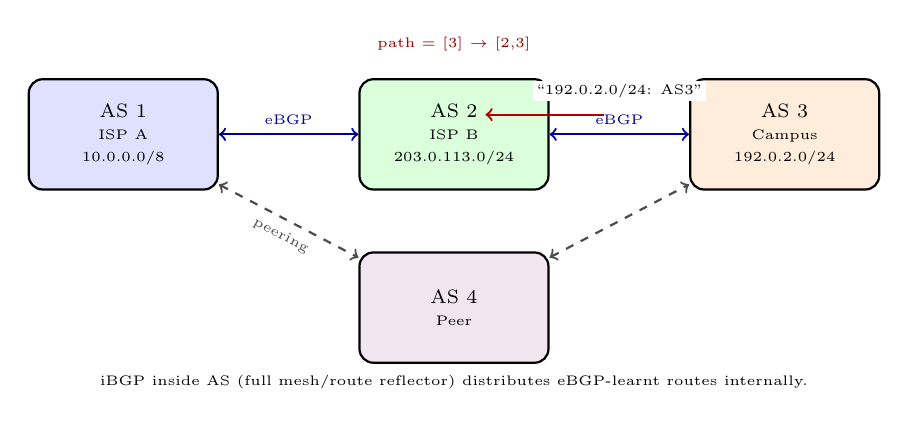
\begin{tikzpicture}[every node/.style={font=\scriptsize},
  as/.style={draw, thick, rounded corners=5pt, minimum width=2.4cm, minimum height=1.4cm, align=center}]
\node[as, fill=blue!12] (as1) at (0,0) {AS 1\\{\tiny ISP A}\\{\tiny 10.0.0.0/8}};
\node[as, fill=green!14] (as2) at (4.2,0) {AS 2\\{\tiny ISP B}\\{\tiny 203.0.113.0/24}};
\node[as, fill=orange!14] (as3) at (8.4,0) {AS 3\\{\tiny Campus}\\{\tiny 192.0.2.0/24}};
\node[as, fill=violet!10] (as4) at (4.2,-2.2) {AS 4\\{\tiny Peer}};
\draw[<->, thick, blue!60!black] (as1) -- node[above, font=\tiny] {eBGP} (as2);
\draw[<->, thick, blue!60!black] (as2) -- node[above, font=\tiny] {eBGP} (as3);
\draw[<->, thick, dashed, gray!60!black] (as1) -- node[below, sloped, font=\tiny] {peering} (as4);
\draw[<->, thick, dashed, gray!60!black] (as4) -- (as3);
\node[font=\tiny, fill=white, inner sep=1pt] at (6.3,0.55) {``192.0.2.0/24: AS3''};
\draw[->, thick, red!70!black] (6.1,0.25) -- (4.6,0.25);
\node[font=\tiny, align=left, red!60!black] at (4.2,1.15) {path = [3] $\to$ [2,3]};
\node[font=\tiny, align=center] at (4.2,-3.15) {iBGP inside AS (full mesh/route reflector) distributes eBGP-learnt routes internally.};
\end{tikzpicture}}%
\caption{BGP inter-domain routing: each AS advertises its prefixes with AS-path. Policy (prefer customer $>$ peer $>$ provider) overrides shortest path; hot-potato forwards to nearest egress.}
\label{fig:bgp-as}
\end{figure}
BGP is \emph{policy}-driven: an AS may prefer a longer customer route over a shorter peer route (economics beats hops). Decision steps: (1) highest local-pref (operator policy), (2) shortest AS-path, (3) lowest MED (hint from neighbour), (4) hot-potato (lowest IGP cost to egress), (5) tie-break router ID. Hot-potato forwards to the closest egress point, even if the AS-path is slightly longer internally.
Inside an AS, iBGP disseminates externally learnt routes and the IGP (OSPF) handles internal hops. Convergence is slow---path exploration after failures can take minutes and cause transient loops. BGP security (prefix hijacks) is a real risk; RPKI/ROA helps authenticate origins.
\section{NAT: One Public Address for a Whole Home}\label{sec:nat}
\emph{Intuition first.} A home router is like an office receptionist with one public phone number: inside, every desk has a short extension (private address); outside callers only see the reception number, and the receptionist routes by extension (port). IPv4 has only $2^{32}\approx4.3$ billion addresses, far too few for every device, so RFC\,1918 reserves private ranges---$10.0.0.0/8$, $172.16.0.0/12$, $192.168.0.0/16$---reusable inside each network but never routed on the public Internet. Your laptop at $192.168.1.10$ keeps that address at home, at NTU, and at a cafe simultaneously; a NAT gateway at the edge translates it to the one globally routable public address the ISP assigned.
NAPT (NAT with port translation, what home routers do) multiplexes many private hosts onto that single public IP by rewriting the source port. Outgoing: $(192.168.1.10{:}5001 \to 142.250.1.1{:}80)$ becomes $(203.0.113.7{:}61001 \to 142.250.1.1{:}80)$, and the gateway records $(61001 \leftrightarrow 192.168.1.10{:}5001)$ in its translation table; a second laptop using the same private port gets a different public port (say $61002$), so the 16-bit port field supplies $\sim$64k concurrent flows per public IP. Incoming replies to $203.0.113.7{:}61001$ are reverse-mapped and forwarded inside; unsolicited inbound packets with no table entry are dropped.
\begin{figure}[h]
\centering
\resizebox{\linewidth}{!}{%
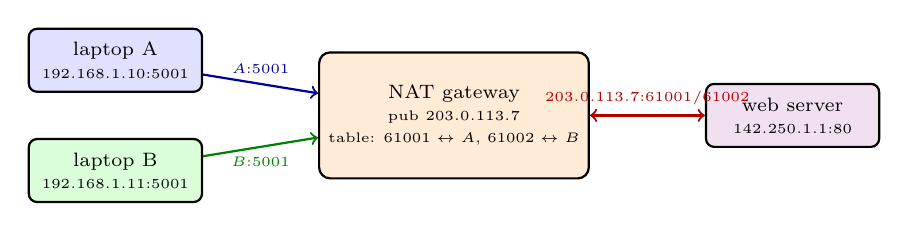
\begin{tikzpicture}[every node/.style={font=\scriptsize}, host/.style={draw, thick, rounded corners=3pt, minimum width=2.2cm, minimum height=0.8cm, align=center}, nat/.style={draw, thick, rounded corners=4pt, minimum width=2.6cm, minimum height=1.6cm, align=center}]
\node[host, fill=blue!12] (h1) at (0,0.7) {laptop A \\ {\tiny $192.168.1.10{:}5001$}};
\node[host, fill=green!14] (h2) at (0,-0.7) {laptop B \\ {\tiny $192.168.1.11{:}5001$}};
\node[nat, fill=orange!16] (ng) at (4.3,0) {NAT gateway \\ {\tiny pub $203.0.113.7$} \\ {\tiny table: $61001 \leftrightarrow A$, $61002 \leftrightarrow B$}};
\node[host, fill=violet!12] (srv) at (8.6,0) {web server \\ {\tiny $142.250.1.1{:}80$}};
\draw[->, thick, blue!60!black] (h1) -- node[above, font=\tiny] {$A{:}5001$} (ng);
\draw[->, thick, green!50!black] (h2) -- node[below, font=\tiny] {$B{:}5001$} (ng);
\draw[<->, thick, red!70!black] (ng) -- node[above, font=\tiny] {$203.0.113.7{:}61001/61002$} (srv);
\end{tikzpicture}}%
\caption{NAPT multiplexes two hosts sharing private port $5001$ onto one public IP via distinct public ports. Return traffic is demultiplexed by table lookup; unsolicited inbound has no entry and is dropped.}
\label{fig:nat}
\end{figure}
Drawback: NAT breaks the end-to-end principle---a host behind NAT has no stable public address, so inbound connections (P2P calls, game hosting, servers) fail without hole-punching (STUN/TURN/ICE), UPnP port-forwarding, or manual rules. Carrier-grade NAT stacks a second translation at the ISP, adding latency and logging burden (abuse traceback needs timestamped port logs). NAT also mangles protocols embedding addresses (classic FTP, SIP), needing application gateways. It was a survival fix for exhaustion, not architecture: the long-term answer is IPv6.
\begin{example}[NAPT walk-through]\label{ex:napt}
Laptops $A=192.168.1.10{:}5001$ and $B=192.168.1.11{:}5001$ both open \texttt{142.250.1.1:80}. Gateway (public $203.0.113.7$) assigns $61001 \leftrightarrow A$, $61002 \leftrightarrow B$ and rewrites sources. Server replies to $203.0.113.7{:}61001$ and $203.0.113.7{:}61002$; the gateway maps each back to the right laptop. Netstat on $A$ still shows $5001$---translation is invisible to endpoints. If the table holds 60k entries and each web page opens 6 flows, one public IP serves $\approx$10k concurrent page loads.
\end{example}
\section{IPv6: More Addresses and a Simpler Header}\label{sec:ipv6}
\emph{Intuition first.} IPv6 keeps IP's forwarding idea but removes the two crutches---private addresses plus NAT, and router fragmentation---by making addresses plentiful and headers router-friendly. Addresses are 128-bit ($2^{128}\approx3.4\times10^{38}$), written as eight hex groups, e.g.\ \texttt{2001:db8:0:0:0:0:0:1}, compressible to \texttt{2001:db8::1} (one \texttt{::} run, leading zeros droppable). A typical home gets a $/64$ (as many addresses as the whole IPv4 Internet squared per subnet); key scopes are global unicast $2000\texttt{::}/3$, link-local \texttt{fe80::/10} (single link, like ARP scope), loopback \texttt{::1}, and multicast \texttt{ff00::/8}. Subnetting works as in IPv4: $/64$ network $+$ $64$-bit interface ID, often auto-configured (SLAAC) from the MAC.
The header is fixed 40\,B (vs.\ variable 20--60\,B): version, traffic class, 20-bit flow label (QoS flows without deep inspection), payload length, next-header (replaces protocol), hop limit (renamed TTL), and 16\,B source/destination. Dropped: header checksum (links already check), IHL/options (moved to chained extension headers: hop-by-hop, routing, fragment, ESP/AH, only processed when present), and router fragmentation (only the source fragments, after Path MTU Discovery; routers send ICMPv6 Packet-Too-Big). Fixed layout means fast hardware parsing; extension chaining keeps the common case cheap.
\emph{Worked micro-example.} Expand \texttt{2001:db8::7} to \texttt{2001:0db8:0000:0000:0000:0000:0000:0007} (eight groups). Under prefix \texttt{2001:db8:abcd::/48}, the first 48 bits are fixed, leaving $2^{80}$ addresses---enough for $2^{16}$ customer $/64$s each holding $2^{64}$ hosts. \emph{Transition:} dual-stack hosts run both protocols (DNS \texttt{A} vs.\ \texttt{AAAA} selects); tunnels (6to4, Teredo) carry v6 over v4; NAT64/DNS64 lets v6-only clients reach v4 servers. Adoption was slow because NAT made v4 ``good enough'' and every middlebox must upgrade---but mobile and cloud growth now push v6 past half of Google traffic.
\section{Putting It Together: A Packet's Life Through the Network Layer}\label{sec:packet-life}
Trace a ping from NTU host \texttt{10.1.2.3/24} to \texttt{203.0.113.10/24} via two routers.
Host checks destination: same prefix? No ($10.1.2.0/24 \neq 203.0.113.0/24$), so it forwards to its gateway \texttt{10.1.2.1}.
It ARPs for the gateway MAC, wraps the IP datagram in an Ethernet frame, and sends.
Router~1 strips the frame, does LPM on \texttt{203.0.113.10}: longest match is \texttt{203.0.113.0/24} $\to$ link~1.
It decrements TTL, recomputes checksum, ARPs for next-hop MAC if needed, and re-encapsulates.
Router~2 repeats LPM and delivers to the subnet; the destination host strips headers and replies.
This hop-by-hop re-wrapping is why IP can run over any link technology.

\begin{remark}[Why best-effort?]
IP deliberately does not retransmit or order packets. Reliability is left to TCP at the edges.
This keeps routers simple and fast---they just forward. Complexity at the edges, simplicity in the core is the end-to-end principle that scaled the Internet.
If IP did reliability, every router would need per-flow state and timers, exploding cost.
\end{remark}

A second example: Path MTU Discovery. Host sends with DF=1 and large size;
a router with MTU 1280 drops it and returns ICMP ``Packet Too Big''
with its MTU. Host lowers size and retries.
No fragmentation occurs, yet delivery succeeds---cooperation
between network (ICMP) and transport/host improves efficiency.

Aggregation examples: two /24s aggregate to a /23 (512 addresses), two /23s to a /22 (1024), and ISP block 	exttt{14.24.0.0/15} holds 131\,072. This hierarchy keeps the global BGP table tractable.
This aggregation principle is applied recursively: RIRs allocate large blocks to ISPs, ISPs sub-allocate to customers, and longest-prefix match ensures the most specific advertisement wins. Without it, the global table would exceed a million entries and exceed router memory.

A practical check: run \texttt{ip route show} on Linux or \texttt{show ip bgp summary} on a Cisco router. You will see prefixes, next-hops, and AS-paths exactly as described.


\section{Chapter Notes}
IPv4 details in RFC\,791, CIDR in RFC\,4632, OSPF in RFC\,2328, BGP-4 in RFC\,4271. Kurose--Ross Ch.~4 and Peterson--Davie give fuller case studies. Dijkstra (1959) and Bellman--Ford (1958) are covered algorithmically in SC2001; here we use them as routing protocols. For hands-on, run \texttt{traceroute} to see TTL in action and \texttt{ip route} to inspect a forwarding table.
\section{Exercises}\label{sec:ch05-exercises}
\begin{enumerate}[label=E5.\arabic*, leftmargin=*, itemsep=0.7em]
    \item \textbf{CIDR and table size.} An ISP owns $14.24.0.0/15$. (a) How many /24 blocks does it contain? (b) If it previously advertised each /24, how many BGP entries does aggregation save? (c) A customer needs 60 hosts; what smallest prefix length suffices and what mask? (d) Why does aggregation not always reduce table size?
    \item \textbf{Longest-prefix match by hand.} Table: $10.0.0.0/8\to0$, $10.1.0.0/16\to1$, $10.1.1.0/24\to2$, $0/0\to3$. For dst $10.1.1.23$, $10.1.2.5$, $192.0.2.1$ give egress link. Draw the binary trie and show how LPM walks it.
    \item \textbf{Dijkstra trace and proof.} Run Dijkstra from $s$ on Fig.~\ref{fig:dijkstra} to completion; list extraction order and final distances to $t$. Prove the invariant: when $u$ leaves the PQ, $\mathit{dist}[u]=\delta(s,u)$. Where does $w\ge0$ get used? Give a counterexample with a negative edge.
    \item \textbf{Count-to-infinity.} Three nodes $a$--$b$--$c$ line ($c=1$ each). Link $b$--$c$ cost $\to\infty$ (failure). Show distance-vector updates without poisoned reverse and count steps to converge (assume infinity = 16). Then show poisoned reverse fixes this case and give a 3-node loop where it still fails.
    \item \textbf{BGP policy vs.\ shortest path.} AS2 learns $192.0.2.0/24$ via AS3 (customer, path [3]) and via AS4 (peer, path [4,3]). Which does BGP prefer under standard customer$>$peer policy? If AS2 forwards via hot-potato, how does internal OSPF cost affect egress choice? Sketch the full decision steps (local-pref, AS-path, MED, IGP cost) and when each applies.
\end{enumerate}
% End of Chapter 5
